\documentclass[border=6pt]{standalone}
\usepackage{tikz}
\usetikzlibrary{arrows.meta,positioning}
\begin{document}
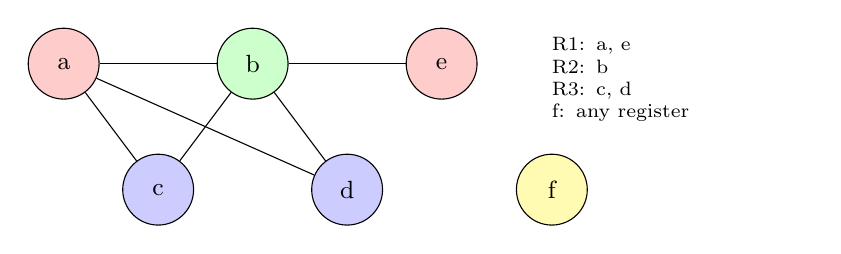
\begin{tikzpicture}[font=\small,
 v/.style={draw,circle,minimum size=0.9cm,inner sep=0pt}]
\node[v,fill=red!20] (a) at (0,1.6) {a};
\node[v,fill=green!20] (b) at (2.4,1.6) {b};
\node[v,fill=blue!20] (c) at (1.2,0) {c};
\node[v,fill=blue!20] (d) at (3.6,0) {d};
\node[v,fill=red!20] (e) at (4.8,1.6) {e};
\node[v,fill=yellow!30] (f) at (6.2,0) {f};
\draw (a)--(b); \draw (a)--(c); \draw (b)--(c); \draw (a)--(d); \draw (b)--(d); \draw (b)--(e);
\node[font=\scriptsize,align=left,text width=3.2cm] at (7.8,1.4) {R1: a, e\\R2: b\\R3: c, d\\f: any register};
\end{tikzpicture}
\end{document}
